\documentclass[12pt]{article}

\usepackage{sbc-template}
\usepackage{graphicx,url}
\usepackage{subcaption}
\usepackage[utf8]{inputenc}
\usepackage[brazil]{babel}

     
\sloppy

%\title{Análise Comparativa de Desempenho em~\emph{drivers} para MongoDB em Aplicações Node.js}
\title{Comparação de Desempenho entre~\emph{Drivers} do MongoDB em Aplicações Node.js}

%\author{Leandro Ungari Cayres, Ronaldo Celso Messias Correia }
\author{Leandro Ungari Cayres, Bruno Santos de Lima, Rogério Eduardo Garcia,\\ Ronaldo Celso Messias Correia}
%\author{OMITIDO}

\address{Faculdade de Ciências e Tecnologia -- Universidade Estadual Paulista (UNESP)\\
  Presidente Prudente -- SP -- Brazil
  %\email{\{leandro.ungari,ronaldo.correia\}@unesp.br}
\email{\{leandro.ungari,bruno.s.lima,ronaldo.correia,rogerio.garcia\}@unesp.br}
}

%\address{OMITIDO\\
%\email{OMITIDO}
%}

\begin{document} 

\maketitle

\begin{abstract}
In recent years, the number of NoSQL database has grown significantly. Such databases do not have a common language for defining and manipulating data, so this role is assigned to APIs or Drivers. There are cases where, for the same database, there are several solutions, which makes it difficult to understand the impacts that the choice of each option has. In this paper, we present a comparative study between two MongoDB Drivers in Node.js applications, in which CRUD operations were performed for performance analysis based in metrics: runtime, CPU and memory consumption. The results demonstrate that, under quantative analysis, MongoClient performs better.
\end{abstract}
     
\begin{resumo} 
Nos últimos anos, o número de banco de dados NoSQL tem crescido significativamente. Tais bases não possuem uma linguagem comum para definição e manipulação dos dados, de modo que esse papel é atribuído a API's ou \emph{Drivers}. Há casos em que, para o mesmo banco de dados, existem diversas soluções, o que dificulta o entendimento dos impactos que a escolha de cada opção tem. Neste artigo, é apresentado um estudo comparativo entre dois \emph{Drivers} para MongoDB em aplicações Node.js, em que foram executadas operações CRUD para análise de desempenho com base em métricas de tempo de execução, consumo de CPU e memória. Os resultados demonstram que, sob análise quantitativa, o \emph{Driver} \emph{MongoClient} tem melhor desempenho.
\end{resumo}


\section{Introdução}
\label{sec:introducao}

Nos últimos anos, o crescimento no volume de dados mudou a utilização desses por empresas e organizações. Inicialmente, os dados eram considerados agentes passivos, relacionados às regras de negócio empresarial; tornaram-se potenciais oportunidades de lucro e obtenção de conhecimento através de processos de análise de informações.

O advento do~\emph{Big Data} não implicou somente em maior espaço de armazenamento, mas em uma mudança de organização, considerando características como volume, variedade, velocidade e valores~\cite{ward2013undefined}. A arquitetura dos tradicionais Bancos de Dados Relacionais são baseadas nas propriedades ACID (\textit{atomicity},~\textit{consistency},~\textit{isolation} e~\textit{durability}), contudo, em ambientes de~\emph{Big Data} a alta consistência provida pelos Bancos de Dados Relacionais, afeta diretamente os aspectos de disponibilidade e eficiência, que são primordiais, devido ao alto volume, variedade e velocidade~\cite{aparicio:2016}. Nesse cenário, os Banco de Dados \textit{NoSQL} (\emph{Not only SQL}) promovem maior flexibilidade estrutural, escalabilidade, suporte a replicação e consistência eventual e surguem como alternativas eficientes.~\cite{han2011survey}. 
 
Diferentemente do modelo relacional, os Bancos de Dados \textit{NoSQL} não possuem uma linguagem semelhante ao SQL (\emph{Structured Query Language})~\cite{bugiotti2013object,sellami2014odbapi}. Desse modo, para os diferentes ambientes de desenvolvimento e linguagens de programação,~\emph{Drivers} tem sido desenvolvidos de modo a viabilizar a execução dos comandos no banco de dados. 

Em muitos casos, os~\emph{Drivers}, além de recentes, apresentam limitações em sua implementações, falhas de entendimento e efeitos colaterais no acesso aos dados~\cite{rafique:2018}. Em muitas situações, a decisão de qual combinação entre Banco de Dados \textit{NoSQL} e~\emph{Driver} a ser empregada pode ser um problema, devido ao desconhecimento dos pontos positivos e negativos de cada combinação.

Neste artigo, por meio de um estudo comparativo de desempenho, busca-se avaliar as duas principais soluções de~\emph{Drivers} para o MongoDB~\footnote{https://www.mongodb.com/}, respectivamente MongoClient~\footnote{https://mongodb.github.io/node-mongodb-native/} e Mongoose~\footnote{https://mongoosejs.com/}, em ambientes de aplicação Node.js. 
O principal fator considerado para a realização dessa análise consiste na definição prévia de esquema para a manipulação dos dados em operações de CRUD (\emph{create}-\emph{read}-\emph{update}-\emph{delete}). Conceitualmente, os Bancos de Dados~\textit{NoSQL} não requerem essa predefinição, proporcionando flexibilidade, entretanto, não existe nada que impeça sua utilização, principalmente quanto a respeito do desempenho; possibilitando algum impacto relevante.

O Banco de Dados MongoDB foi escolhido devido a sua enorme popularidade recente, empregado em diversas aplicações e pesquisa~\cite{patil:2017,jung:2015,ongo:2018,kanade2014study}; e uma das principais opções de armazenamento orientada a documentos. Quanto ao Node.js, mesmo recente, alguns trabalhos apontam a sua viabilidade tecnológica no desenvolvimento de aplicações~\cite{chaniotis2015node}. Com essa escolha, tanto aplicação quanto banco de dados utilizam \textit{JavaScript}, uniformizando o sistema em termos de linguagem de programação.

O restante desse artigo está organizado do seguinte modo: na Seção~\ref{section:fundamentacao} são apresentados conceitos de Banco de Dados NoSQL, MongoDB e seus \emph{Drivers}, além do ambiente de execução Node.js. 
A Seção~\ref{section:experimento} é apresentada a estruturação do experimento. 
Na Seção~\ref{section:resultados} são descritos os resultados quantitativos obtidos, cuja discussão está situada na Seção~\ref{section:discussao}. Na Seção~\ref{section:relacionados} relata os trabalhos relacionados. Por fim, a Seção~\ref{section:consideracoes} expressa as considerações finais e perspectivas de trabalhos futuros.

\section{Fundamentação Teórica}
\label{section:fundamentacao}

Nesta seção, são discutidos alguns conceitos fundamentais para o trabalho: Bancos de Dados NoSQL, as características do MongoDB e dos \emph{Drivers} MongoClient e Mongoose, organização de aplicações Node.js. 

\subsection{Banco de Dados NoSQL}
\label{subsection:nao-relacional}

Os bancos de dados NoSQL, foram desenvolvidos visando armazenar e processar grandes volumes de dados. Em linhas gerais os bancos de dados NoSQL são livres de esquematizações e mais propícios a lidar com dados não estruturados como e-mails, documentos e mídias sociais de maneira eficiente~\cite{mohamed:2014,ramesh:2016}.

O termo NoSQL é utilizado para se referir a uma ampla variedade de armazenamentos de dados, em que as restrições de transação ACID foram suavizadas permitindo melhor dimensionamento e desempenho horizontal~\cite{rafique:2018}, proporcionando esquemas menos estruturados, suporte a operações de junção, alta escalabilidade, modelagem de dados simples com linguagem de consulta simples~\cite{ramesh:2016}. Os bancos de dados NoSQL são categorizados em: armazenamento de documentos, famílias de colunas, chave/valor, grafos e multimodais~\cite{aparicio:2016}.

Este trabalho tem como foco a categoria orientada a documentos, a qual possui modelagem de dados estreitamente relacionados a programação orientada a objetos, os quais possibilitam flexibilidade no armazenamento de registros  com atributos distintos, sendo útil na modelagem de dados não-estruturados e polimórficos. Essa categoria permite consultas robustas, em que qualquer combinação de campos no documento pode ser realizada visando consultar dados~\cite{patil:2017}. Os dados são organizados em coleções de documentos, as quais utilizam uma estrutura semelhante a JSON (\emph{JavaScript Object Notation}) ou XML (\emph{Extensible Markup Language}).

\subsection{MongoDB}

O MongoDB é um Banco de Dados orientado a documentos que possui código-aberto, provendo funcionalidades como ordenação, indexação secundária e consultas de intervalo~\cite{membrey2011definitive}.
 
O banco de dados não impõe um esquema prévio, entretanto, normalmente todos os documentos em uma coleção são de propósito semelhante ou relacionado~\cite{kanade2014study,lutu2015big}. Há duas abordagens para modelagem de documentos:

\begin{itemize}
\item \textbf{Modelo de dados incorporado:} Os dados relacionados são incorporados em uma única estrutura ou documento. Esses esquemas são geralmente conhecidos como modelos sem normalização. %REFERENCIAR
\item \textbf{Modelo de dados normalizado:} Os dados possuem referências de documentos para registrar relacionamentos entre esses, mas a combinação de documentos deve ser feita diretamente no código-fonte da aplicação. %REFERENCIAR
\end{itemize}

O armazenamento dos dados ocorre através da serialização de objetos Javascript, também conhecidos como JSON, cuja implementação interna utiliza uma codificação binária chamada BSON\footnote{http://bsonspec.org/}. O banco de dados MongoDB disponibiliza diversos~\emph{Drivers} para linguagens de programação como Java, C++, C\#, PHP e Python~\cite{lutu2015big}, e também em Node.js.

%O QUE SÃO DRIVERS PARA UM BD? QUAL CONTEXTO?
Nesse contexto, dentre os~\emph{Drivers} existentes, tem-se como destaque o \textbf{\textit{MongoClient}}\footnote{https://mongodb.github.io/node-mongodb-native/index.html}, consiste na solução oficial e nativa provida organização, provendo um conjunto de funcionalidades que permite a manipulação dos dados e uso de recursos avançados do sistema. Essa solução é caracterizada pela modelagem documentos-objeto (\emph{ODM -- Object-Document Modeler}) de modo implícito ao banco de dados.

Assim como o anterior, o \textbf{\textit{Mongoose}} consiste também em um \emph{Driver} para MongoDB, em que provê a modelagem de dados utilizando um mecanismo objeto-relacional (\emph{ORM -- Object Relational Mapping}) utilizado em banco de dados relacionais~\cite{mardan2014boosting}, executando diversas tarefas de verificação e validação dos dados, como nulidade ou tipagem, previamente definidos por meio da elaboração de um esquema.

\subsection{Node.js}
\label{subsection:nodejs}

Node.js é uma plataforma construída sob o ambiente de execução para JavaScript do navegador Google Chrome, para criação facilitada de aplicações de internet rápidas e escaláveis, baseado em um mecanismo orientado a eventos de entrada e saída não-bloqueante, que viabiliza a interação do usuário enquanto demais tarefas executam em segundo-plano, resultando em aplicações leves e eficientes.
Cada aplicação Node.js atua como processo comum em um computador, diferentemente da restrição de aplicações JavaScript voltadas para navegadores. A Figura~\ref{figure:memoria} apresenta a organização da memória em processos Node.js.

\begin{figure}[!h]
    \centering
    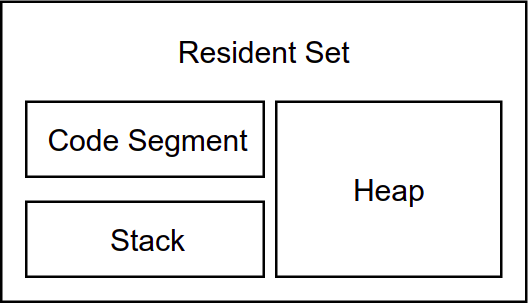
\includegraphics[width=0.35\textwidth]{images/set}
    \caption{Organização de memória de um processo Node.js -- Adaptado de~\cite{nodememory}.}
    \label{figure:memoria}
\end{figure} 

A região principal é chamada~\emph{Resident Set}, a qual corresponde a toda memória utilizada no processo. Em seguida, tem-se a região~\emph{Code Segment}, a qual armazena todas as instruções definidas para o programa. A próxima região~\emph{Stack} armazena todas as variáveis e estruturas de dados utilizadas durante o tempo de vida dessas. Por fim, tem-se a região~\emph{Heap}, a qual armazena dados específicos como objetos, strings e closures; em geral, cada processo aloca esse região com um tamanho predefinido, contudo essa pode ser utilizada apenas parcialmente ou em sua totalidade~\cite{nodememory}. 

\section{Composição do Experimento}
\label{section:experimento}

Nesta seção é apresentado a composição do experimento comparando os~\emph{Drivers} MongoClient e Mongoose em integração com o MongoDB. 
Na Figura~\ref{figure:diagrama-banco} é ilustrado a esquematização do experimento. 

\begin{figure}[!ht]
    \centering
    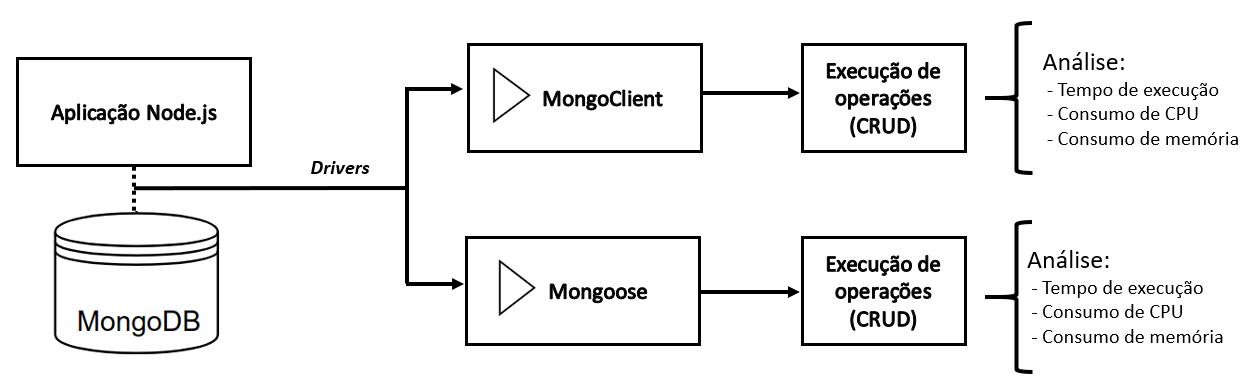
\includegraphics[width=\textwidth]{images/esquema-experimento.png}
    \caption{Experimento: Comparação entre os \emph{Drivers} do MongoDB.}
    \label{figure:diagrama-banco}
\end{figure}
 
Neste estudo, foram conduzidas análises visando identificar qual dupla (MongoDB e \emph{Drive}) possui melhor desempenho em uma aplicação Node.js. 
Além disso, foi investigado se o tamanho médio de cada registro presente no conjunto de dados pode influenciar e qual a proporção desse impacto.

Uma aplicação Node.js foi implementada para a condução dos testes, responsável por realizar a conexão com o Banco de Dados MongoDB e executar as operações CRUD. A ferramenta de testes implementada em Node.js está disponível em: [OMITIDO].%~\footnote{https://github.com/leandroungari/database-driver}.

As métricas escolhidas para análises de cada um dos testes conduzidos foram:

\begin{itemize}
\item \textbf{Tempo médio de Execução:} Consiste tempo médio total de execução de cada operação específica.
\item \textbf{Consumo médio de CPU:} Consiste no tempo médio de uso do processador durante a execução da operação específica.
\item \textbf{Consumo médio de Memória:} Consiste na variação média de uso de memória RAM durante a execução da operação específica, sendo expressa em kilobytes (KB).
\end{itemize}

Por fim, foram formuladas as seguintes de questões de pesquisa que guiaram formalmente as análises executadas: 

\textbf{Q1} --~\emph{A escolha do driver impacta no tempo de execução de cada uma das operações de CRUD?}

\textbf{Q2} --~\emph{A escolha do driver pode influenciar no tempo de processamento (CPU) nas operações de CRUD?}

\textbf{Q3} --~\emph{A escolha do driver impacta de modo relevante quanto ao uso de memória nas operações de CRUD?}

\subsection{Características dos Conjuntos de Dados}

A condução do experimento utilizou um conjunto de dados com cerca 18 mil instâncias.%\footnote{https://www.kaggle.com/karangadiya/fifa19}. 
Originalmente, todos os registros presentes são compostos por 89 atributos, predominantemente textuais, obtendo um tamanho médio de 1,37KB. 
A partir do conjunto original, foi construído um conjunto reduzido em número de atributos (6 atributos), com o mesmo total de instâncias, porém com tamanho médio de 0,13KB. 

Deste modo, dois conjuntos de dados foram utilizados para a experimentação, observe a Tabela~\ref{tab:conjunto-dados}. 
O conjunto reduzido tem o intuito de comparar os dois \emph{Drivers} na manipulação de registros com diferentes quantidade de atributos.

\begin{table}[ht]
\centering
\caption{Características dos Conjuntos de Dados utilizado no Experimento}
\label{tab:conjunto-dados}
\begin{tabular}{c|c|c|}
\cline{2-3}
                         & \textbf{Conjunto de Dados 1} & \textbf{Conjunto de Dados 2} \\ \hline
\multicolumn{1}{|l|}{Quantidade de instâncias} & 18 mil   		 			& 18 mil            \\ \hline
\multicolumn{1}{|l|}{Quantidade de atributos}  & 89        		 			& 6                  \\ \hline
\multicolumn{1}{|l|}{Tamanho de um registro}   & 1,37 KB        				& 0,13 KB                    \\ \hline
\end{tabular}
\end{table}

\subsection{Ambiente de Execução}

O ambiente de execução foi composto por uma máquina com Ubuntu 18.04.2 OS, processador Intel i3 3217U e memória RAM de 4GB DDR3. 
Durante a execução dos testes, o ambiente de execução da aplicação Node.js foi definido o uso do~\emph{heap} de memória com limite máximo de 3GB, desse modo restringindo o máximo de operações de cada teste.

Em cada cenário de execução, foram extraídos dados relativos ao tempo de execução, tempo de uso de CPU e uso de memória RAM. 
Foram analisados cenários com diferentes quantidades de operações CRUD, as quais variaram de 1000, 10000, 100000 e 200000; cada qual repetido 10 vezes e registrada a média das execuções. A obtenção das métricas de desempenho foi realizada através da biblioteca JSMeter~\footnote{https://github.com/wahengchang/js-meter}. 

\section{Resultados do Experimento}
\label{section:resultados}

Todos os resultados a seguir são apresentados sob a perspectiva que cada uma das operações CRUD, em que 100\% dos registros são atingidos em cada operação. 
Cada resultado refere-se a uma operação específica, da combinação de um~\emph{Driver} com o  conjunto de dados grande (com todos atributos) ou conjunto de dados pequeno (com número reduzido de atributos) .

\begin{figure}[!ht]
\centering
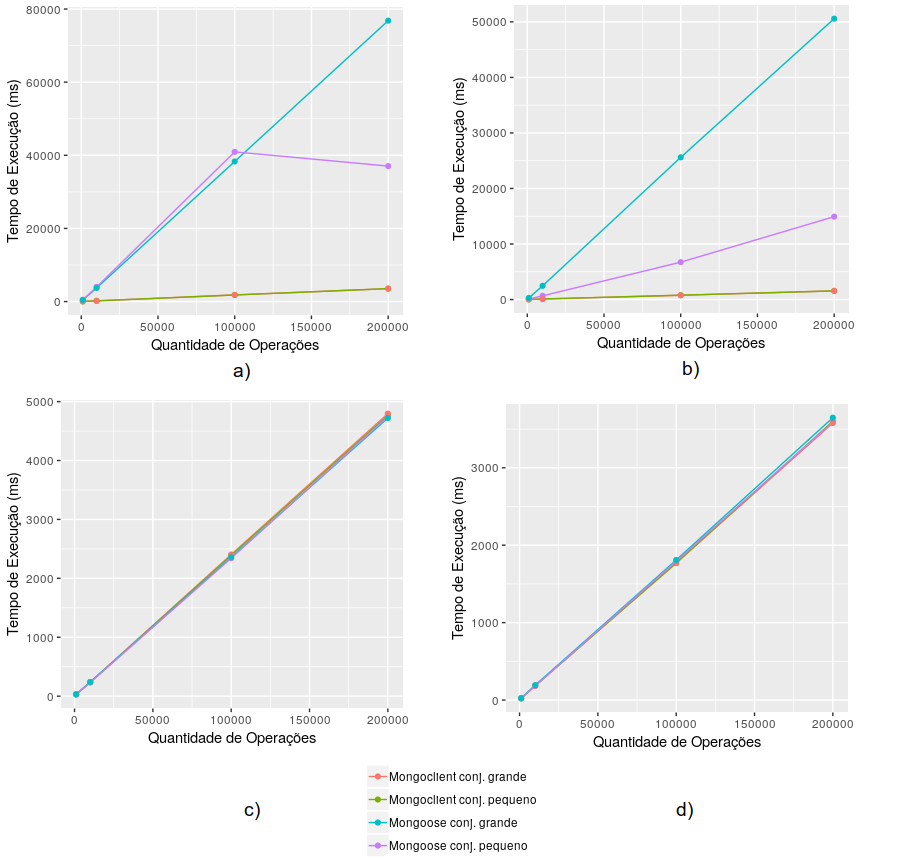
\includegraphics[width=\textwidth]{images/time}
\caption{Comparativo de operações em relação ao tempo de execução.}
\label{fig:time}
\end{figure}

A Figura 3a apresenta, para operação de inserção, o tempo de execução do~\emph{Driver} Mongoose maior, para os dois conjuntos, de modo relevante, enquanto para o MongoClient, aparenta não haver diferenças significativas entre os conjuntos. 
Como exceção, pode-se observar a execução do conjunto pequeno para o Mongoose, em que o tempo para 200 000 operações não mantém a proporcionalidade das demais execuções. Um possível fator que justifique esse comportamento consiste na ocorrência de divisão de conjuntos na operação de inserção quando a quantidade excede 100 000 itens, contudo, isso não ocorre para o conjunto de registros grandes.

A Figura 3b também apresenta, para operação de busca, o tempo de execução inferior para ambos os conjuntos do MongoClient, em que ambos atuam de modo estritamente similar. 
Quanto ao Mongoose, as execuções para conjunto reduzido e grande apresentam comportamento crescente e proporcional em detrimento a diferença de tamanho dos registros. 

As Figuras 3c e 3d, para as operações de atualização e deleção de registros, ambos os~\emph{Drivers} para os conjuntos obtiveram tempos de execução estritamente similares e proporcionando a quantidade de operações, não apresentando diferenças significativas, nem mesmo quanto ao tamanho médio dos registros.

\begin{figure}[!ht]
    \centering
    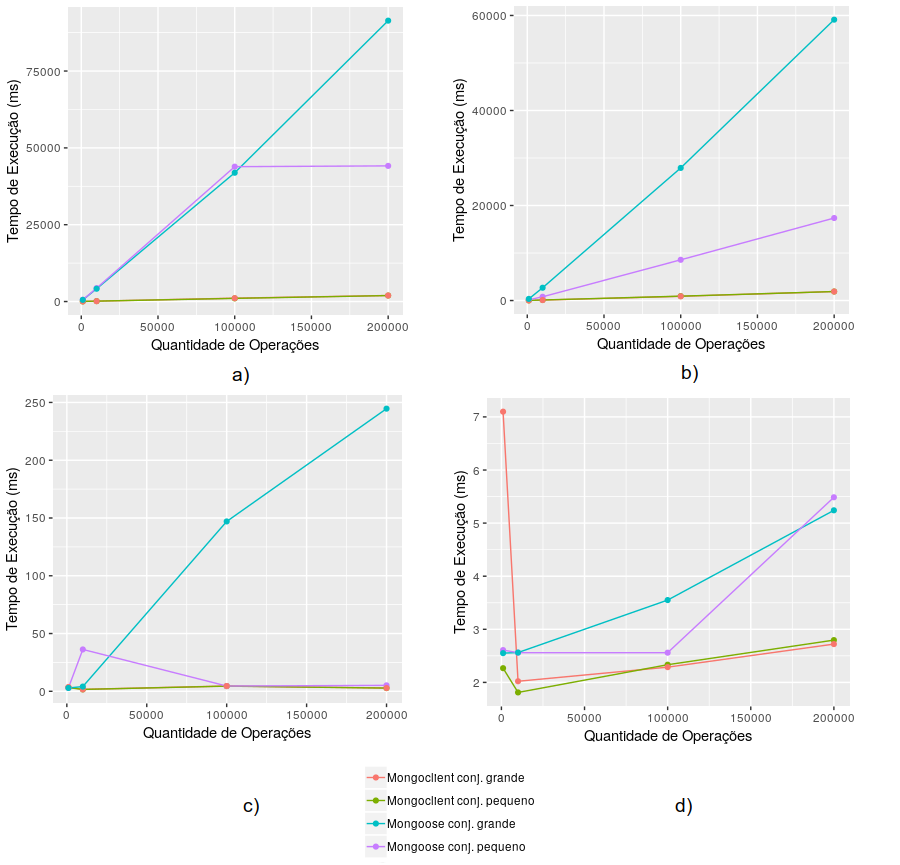
\includegraphics[width=\textwidth]{images/cpuusage}
    \caption{Comparativo de operações em relação ao tempo de uso do processador.}
    \label{fig:cpuusage}
\end{figure}

A próxima análise, na Figura~\ref{fig:cpuusage}, é referente aos resultados relacionados ao tempo de uso de processamento em cada operação.
As Figuras 4a e 4b, assim como análise anterior, para as operações de inserção e busca, apresenta o MongoClient com tempo de execução médio significativamente inferior, em ambos os conjuntos, em detrimento do alto tempo apresentado pelo Mongoose.
Para a inserção, também apresenta o caso de exceção para 200 000 operações, cuja possível justificativa é semelhante a análise anterior.

A Figura 4c, representa a operação de atualização, em que se pode-se observar somente o~\emph{Driver} Mongoose com conjunto de registros maiores apresentou maior tempo de uso de processamento, em detrimento dos demais, que foram semelhantes e com tempo menor, mesmo com oscilações. 
É importante salientar que o tempo de processamento de todas as execuções foram inferiores a 250 ms.
A Figura 4d, representa a operação de deleção, cada execução apresentou comportamento relativamente instável, tendo as execuções com~\emph{Driver} com tempo um pouco maior, contudo não há diferença significativa, porque todas as execuções obtiveram tempo de processamento inferior a 10 ms.

\begin{figure}[!ht]
    \centering
    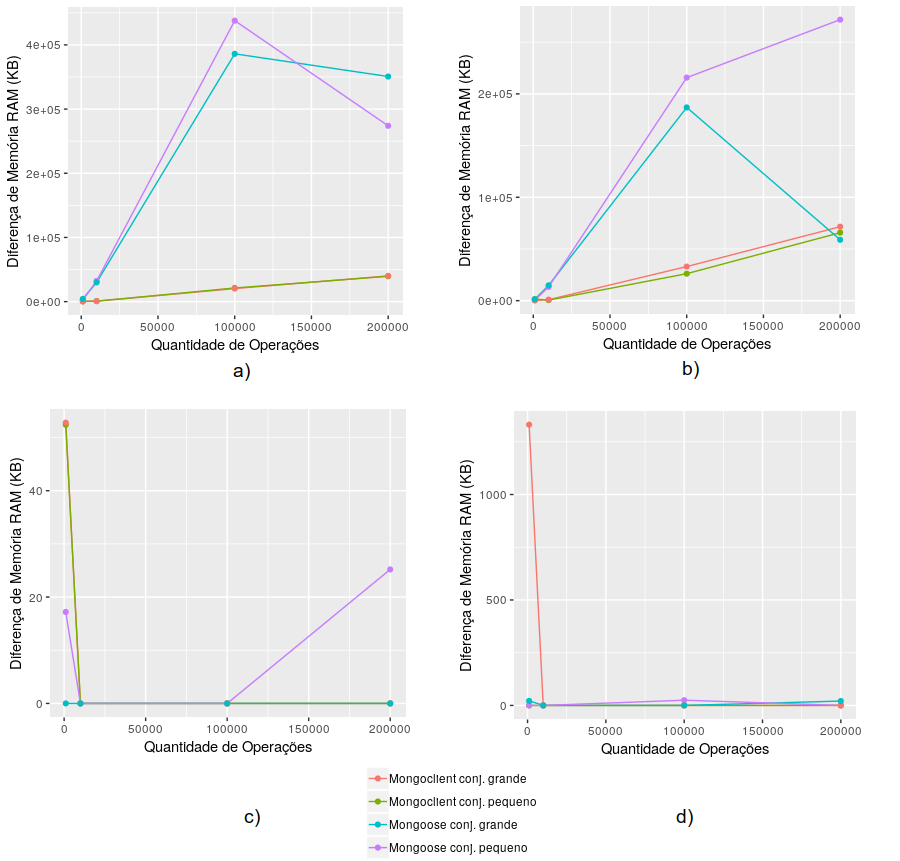
\includegraphics[width=\textwidth]{images/memory}
    \caption{Comparativo de operações em relação ao uso de memória.}
    \label{fig:memory}
\end{figure}

A última análise, apresentada na Figura~\ref{fig:memory}, refere-se a variação média do uso de memória RAM em cada operação.
As Figuras 5a e 5b apresentam o uso de memória para as operações de inserção e busca, no qual não pode se identificar um padrão de uso de memória, contudo pode-se identificar que predominantemente o~\emph{Driver} Mongoose tem um consumo maior de memória na operação realizada, em ambos os conjuntos, em detrimento ao casos do~\emph{Driver} MongoClient.
Para ambas operações, há um uso adicional de memória em torno de 30 a 40MB.

Por fim, as Figuras 5c e 5d, respectivamente operações de atualização e deleção, também não apresentam padronização no consumo de memória para ambos os~\emph{Drivers} e conjuntos. 
Apesar de apresentar alguns pontos de instabilidade, é possível notar que tais operações consomem pouca memória adicional, aproximadamente 1MB ou menos, mesmo considerando os picos de oscilação.

\section{Discussão}
\label{section:discussao}

Nessa seção são apresentadas discussões a respeito dos resultados obtidos, os quais são analisados sob as perspectivas das questões de pesquisa nas Seções~\ref{q1},~\ref{q2} e~\ref{q3}, seguido de uma perspectiva geral do estudo na Seção~\ref{qgeral}.

\subsection{Discussão -- Q1}
\label{q1}

Para a primeira questão de pesquisa, em linhas gerais, os conjuntos executados utilizando o~\emph{Driver} Mongoose apresentaram tempo superior ao MongoClient em duas operações, enquanto nas demais operações obteve resultado semelhante, sem diferenças significativas.
Desse modo, sob a perspectiva de tempo médio de execução de cada operação, temos que, a escolha do~\emph{Driver} pode impactar no desempenho, tendo o MongoClient como melhor opção sob a perspectiva analisada.

\subsection{Discussão -- Q2}
\label{q2}

De modo predominante, assim como na questão anterior, os conjuntos executados utilizando o MongoClient obtiveram melhor tempo de processamento em relação ao Mongoose, em ambos os conjuntos, principalmente para as operações de inserção e busca, enquanto nas demais operações (atualização e deleção), também foi registrado melhor desempenho, contudo em proporção menor.
Em suma, em termos de tempo de processamento, temos que, a escolha do~\emph{Driver} pode influenciar no desempenho, também apresentando MongoClient como melhor opção.

\subsection{Discussão -- Q3}
\label{q3}

A respeito a última questão de pesquisa, tem-se que para as operações de inserção e busca, para a maioria dos casos de execução, o~\emph{Driver} Mongoose apresenta maior consumo de memória, enquanto para as operações de atualização e deleção não há diferenças significantes.
Contudo cabe ressaltar que em nenhuma das comparações houve comportamento estável e proporcional.
Desse modo, em termos de consumo de memória, temos que, a escolha do~\emph{Driver} não impacta de modo relevante para todas as operações, apesar do consumo inferior por parte do~\emph{Driver} MongoClient.

\subsection{Discussão Geral}
\label{qgeral}

De modo geral, os dados obtidos indicam que as operações de inserção e busca são as mais custosas quanto ao tempo de execução, para os piores casos, aproximadamente 70 000 a 80 000 ms, enquanto as demais são inferiores a 5 000 ms.
Sob a perspectiva de tempo de uso de CPU também se vale a mesma análise, inclusive as operações indicam aproximada proporcionalidade em comparação ao tempo de execução total.
Quanto ao uso de memória, ambas operações também apresentam maior custo, mesmo que não-linear, em níveis próximos de 30 a 40MB, em detrimento das demais operações com uso próximo ou inferior a 1MB.

A respeito da diferença média de tamanho dos registros do conjunto de dados adotado, o~\emph{Driver} MongoClient apresentou-se de modo indiferente, não apresentando oscilações significativas, enquanto o Mongoose apresenta o desempenho diretamente proporcional ao tamanho do registro.

Em termos de comparação entre os~\emph{Drivers}, o MongoClient apresentou desempenho mais estável e de menor custo sob a perspectiva de todas as métricas adotadas, em detrimento ao MongoClient.

Portanto, conclui-se que, sob o critério exclusivo de desempenho, o~\emph{MongoClient} apresenta melhor desempenho em relação ao concorrente.
Cabe ressaltar que se quaisquer recursos adicionais providos por uma das opções, como verificação de dados ou facilidade de implementação, consistirem em fatores relevantes, deve-se reavaliar a escolha, contudo, esse estudo tem caráter quantitativo e não visa mensurar a utilização de recursos adicionais que podem variar de contexto e aplicação utilizados.

%\section{Ameaças à Validação}
%\label{section:limitacoes}

%Esta seção apresenta as possíveis ameaças que podem comprometer os resultados desse estudo comparativo.
%Como ameaça à validação interna desse estudo tem a etapa da obtenção dos dados quantitativos quanto às análises conduzidas, desse modo, durante a execução dos testes, todos esses foram conduzidos repetidamente e de modo subsequente para que nenhuma interferência pudesse ser adicionada.

%Como ameaça à validação externa, tem-se o conjunto de dados selecionado, o qual está diretamente atrelado aos resultados numéricos obtidos, porém análise é baseado na comparação relativa dos resultados, além a aplicação de teste foi projetada de modo aceitar um conjunto de dados genérico.

\section{Trabalhos Relacionados} 
\label{section:relacionados}

Com a crescente utilização dos Bancos de Dados NoSQL, \cite{patil:2017} realizou uma análise quantitativa de desempenho entre o MongoDB e o Banco de Dados Relacional MySQL. Como resultados, foi constatado que o MongoDB apresentou melhor performance em operações de inserção e recuperação se comparado com o MySQL. Em um estudo análogo~\cite{jung:2015}, foi demonstrado que o MongoDB possui em geral desempenho superior ao Banco de Dados Relacional PostgreSQL, considerando operações CRUD, entretanto o desempenho do PostgreSQL é superior quando é utilizado um modelo de dados estruturado.

Em outro estudo, \cite{ongo:2018} por meio de uma aplicação web compara o desempenho da utilização integralmente do MySQL e de um modelo híbrido de MySQL e MongoDB. Em seus resultados, é expresso que o banco de dados híbrido obteve desempenho mais alto em operações de leitura e gravação se comparado ao MySQL sozinho. Além disso, o modelo híbrido consome menos disco, contudo consome mais memória se comparado com a utilização integral do MySQL, o consumo de CPU não apresenta diferença significativa entre as duas abordagens. Um possível trabalho futuro poderia comparar o modelo Híbrido com a utilização integralmente do MongoDB e investigar o desempenho, consumo de Disco, Memória RAM e CPU.

\cite{kanade2014study} verificaram a variação do desempenho do Banco de Dados NoSQL MongoDB na perspectiva de dois estilos de modelagem diferentes: incorporação de documentos e normalização em coleções. Os resultados demonstraram que o modelo de dados incorporado do MongoDB oferece um desempenho superior e muito mais consistente em todas as consultas em comparação com o modelo de dados normalizado do MongoDB.

Este trabalho também busca analisar o desempenho do Banco de Dados NoSQL MongoDB considerando tempo de execução, consumo de CPU e Memória. Contudo, diferentemente dos trabalhos presentes na literatura até o momento, buscou-se identificar se a utilização de diferentes \emph{Drivers} do Banco de Dados NoSQL MongoDB pode influenciar no desempenho do mesmo, e caso exista essa influência qual dos~\emph{Drivers} possibilita um maior desempenho considerando operações CRUD.

\section{Considerações Finais}
\label{section:consideracoes}

Este artigo apresenta um estudo comparativo entre~\emph{Drivers} para banco de dados MongoDB.
Na avaliação foram conduzidas análises quantitativas quanto a tempo de execução, tempo de processamento e uso de memória para as operações de CRUD; além de comparar o impacto da variação do tamanho médio dos registros.

De modo geral, através dos resultados quantitativos, foi obtido que o~\emph{Driver} MongoClient obtém melhor desempenho médio quanto a todos as operações, principalmente sob as métricas de tempo de execução e processamento, e, de modo menos significativo, quanto ao consumo de memória.

Adicionalmente, como contribuição adicional deste trabalho, tem-se a implementação da ferramenta de testes, de modo a viabilizar a execução de futuras análises em ambientes Node.js.


\bibliographystyle{sbc}
\bibliography{sbc-template}

\end{document}
